\documentclass[12pt]{article}
\usepackage[tmargin=1.5in]{geometry}
\usepackage{relsize}
\usepackage{babel}
\usepackage{listings}
\usepackage{amsmath}
\usepackage{amssymb}
\usepackage[table]{xcolor}
\usepackage[pdftex]{graphicx}
\usepackage{caption}

\setlength{\parindent}{0cm}  % Indentation prohibited by default
% \captionsetup[figure]{labelformat=empty}    % Remove figure labels

\title{Aufgabenblatt 6: MPI-Prozesse}
\author{Gruppe: CaesarBaurMueller}
\date{\today}

\begin{document}
\maketitle

\begin{sloppypar}
    
\section*{Aufgabe DDT}
\subsubsection*{Wie kann man in DDT die Programmparameter angeben?}
Man kann entweder das Programm ohne Parameter starten und dann in der GUI von DDT die Parameter manuell setzen, oder die Parameter beim Programmaufruf über die Konsole angeben. \\
Ein Beispielaufruf könnte wie folgt aussehen: \verb|ddt -np 4 ./timempi|\\

\begin{figure}[htbp]
    \caption{DDT mit verschiedenen Parametern}
    \begin{minipage}[t]{0.5\textwidth}
        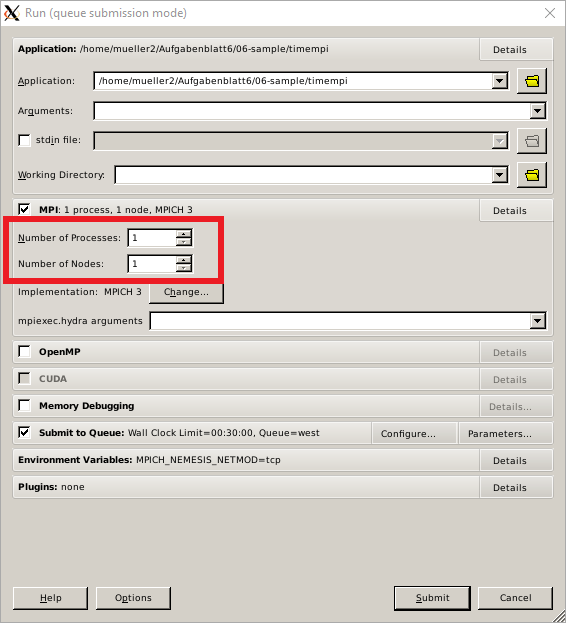
\includegraphics[width=\textwidth]{res/ddt-no-parameter.PNG}
        \caption*{DDT ohne Parameter}
    \end{minipage}
    \begin{minipage}[t]{0.5\textwidth}
        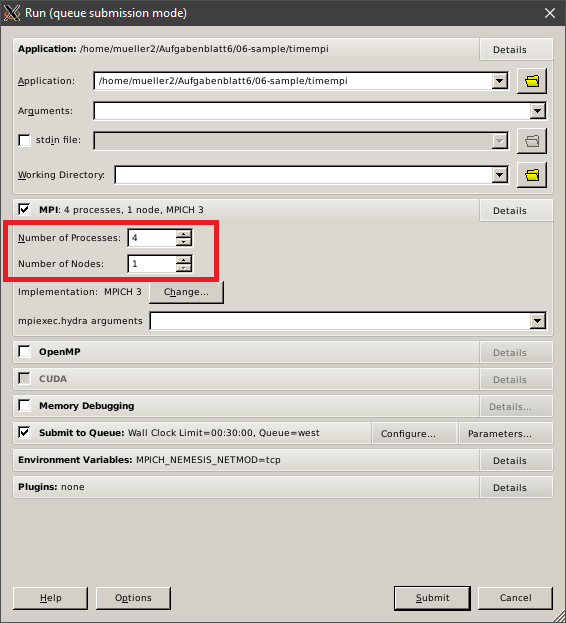
\includegraphics[width=\textwidth]{res/ddt-with-parameter.PNG}
        \caption*{DDT mit Parameter -np 4}
    \end{minipage}
\end{figure}


\subsubsection*{Breakpoints}
Um einen Breakpoint zu setzen muss man in der gewählten Zeile, links neben die Zeilennummer klicken. Dann erscheint dort ein roter Kreis. Dieser zeigt an, dass ein Breakpoint gesetzt wurde. \\
Um nun durch das Programm zu "steppen" gibt es drei Möglichkeiten:
\begin{itemize}
    \item \verb|Step Over|: Führt die aktuelle Zeile aus und springt dann zur nächsten Zeile, die nicht in einer Funktion aufgerufen wird.
    \item \verb|Step Into|: Führt die aktuelle Zeile aus und springt dann in die Funktion, die in der aktuellen Zeile aufgerufen wird, sofern es eine solche gibt. Sonst ist diese Funktion identisch mit \verb|Step Over|.
    \item \verb|Step Out|: Geht im Stack einen Schritt zurück und führt dann die nächste Zeile aus. 
\end{itemize}

\begin{figure}[htbp]
    \centering
    \caption{Step Optionen in DDT}
    \begin{minipage}[t]{0.8\textwidth}
        
\includegraphics[width=\textwidth]{res/ddt-steps.PNG}
        \caption*{Von Links nach Rechts: Step Into, Step Over, Step Out}
    \end{minipage}
\end{figure}


\subsubsection*{Variablen zur Laufzeit}
In DDT lassen sich die Variablen zur Laufzeit betrachten. Hierfür gibt es eine View namens \verb|Locals|, welche sich standardmäßig am rechten Fensterrand befindet. Diese View zeigt alle Variablen an, die im aktuellen Stackframe definiert sind. \\
In dieser View findet sich die Variable \verb|rank| (sobald die sie im Debugger gesetzt wurde). Sie hat je nach Prozess einen anderen Wert (nämlich den Rang des Prozesses). Links neben dem Wert, ist eine Abbildung zu sehen, welche vier Striche enthält die von Links nach Rechts treppenförmig angeordnet sind (Siehe Abb. DDT-View "Locals"). \\
Diese Striche stellen den Werte der Variable in den verschiedenen Prozessen. Wenn wir statt vier, acht Prozesse starten, werden dementsprechend acht Striche angezeigt. \\
Die konkreten Werte der Variable in den verschiedenen Prozessen lassen sich durch einen Klick auf die Striche einsehen. Hier sehen wir in diesem Fall, dass die Variable die jeweilige Prozessnummer/ProzessID darstellt. \\

\begin{figure}[htbp]
    \caption{DDT-View "Locals"}
    \begin{minipage}[t]{0.45\textwidth}
        \vspace{0pt}
        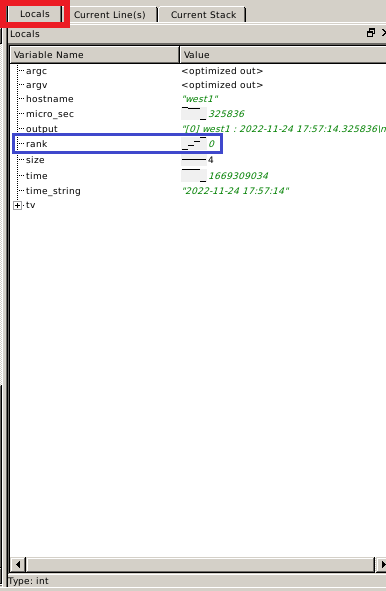
\includegraphics[width=\textwidth]{res/ddt-view-locals.PNG}
        \caption*{Rot: Der Reiter "Locals", Blau: Die Variable "rank"}
    \end{minipage}
    \hspace{0.05\textwidth}
    \begin{minipage}[t]{0.45\textwidth}
        \vspace{0pt}
        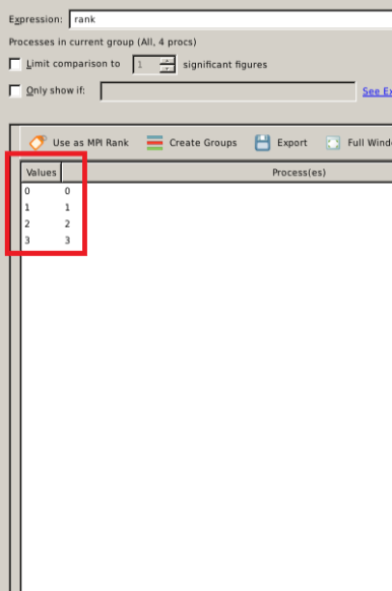
\includegraphics[width=\textwidth]{res/ddt-view-rank.PNG}
        \caption*{Die Werte von "rank" der verschiedenen Prozesse.}
    \end{minipage}
\end{figure}


\subsubsection*{Das Evaluate Fenster}
Das Evaluate Fenster ist eine Live-Ansicht auf die Werte einiger ausgewählter Variablen über alle Prozesse. Es befindet sich standardmäßig unten rechts im Fenster. \\
Zu überwachende Variablen können mit Rechtsklick->"Add Expression" hinzugefügt werden. \\
Auch hier wird eine Grafik mit Strichen angezeigt, welche die Werte der Variablen in den verschiedenen Prozessen darstellen. Als konkreter Variablenwert wird der Wert des aktuell ausgewählten Prozesses angezeigt. Auffällig ist hier, dass es Variablen geben kann die in einigen Prozessen nicht definiert sind. Dies wird dadurch gekennzeichnet, dass der Strich (für den Teil des Prozesses) rot eingefärbt ist. Zudem wird als Variablenwert der Text "$<$No Symbol $<$var$>$ in current context.$>$ angezeigt". Ist die Variable definiert, ist der Strich grün und es wird normal der Variablenwert angezeigt. \\
Dieses Verhalten wird bestätigt, wenn man in der oberen Leiste zwischen den Prozessen hin und her springt.

\begin{figure}[htbp]
    \caption{DDT-View "Evaluate"}
    \begin{minipage}[t]{\textwidth}
        \begin{minipage}[t]{0.5\textwidth}
            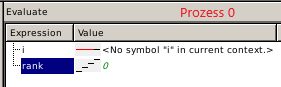
\includegraphics[width=\textwidth]{res/ddt-evaluate-0.PNG}
        \end{minipage}
        \begin{minipage}[t]{0.5\textwidth}
            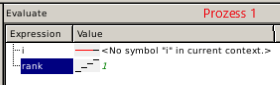
\includegraphics[width=\textwidth]{res/ddt-evaluate-1.PNG}
        \end{minipage}
    \end{minipage}

    \begin{minipage}[t]{\textwidth}
        \begin{minipage}[t]{0.5\textwidth}
            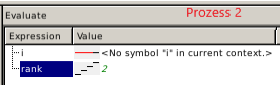
\includegraphics[width=\textwidth]{res/ddt-evaluate-2.PNG}
        \end{minipage}
        \begin{minipage}[t]{0.5\textwidth}
            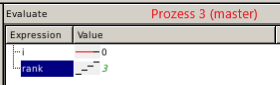
\includegraphics[width=\textwidth]{res/ddt-evaluate-3.PNG}
        \end{minipage}
    \end{minipage}
\end{figure}


\subsubsection*{Datenvisualisierung}
Wir haben in DDT jeweils ein 1D-array, ein 2D-Arrray und ein 3D-Array visualisiert. Dabei sind wir auf das Problem gestoßen, dass das Programm in der Visualisierung extrem langsam ist (lagged). Dadurch konnten wir leider die visuellen Feinheiten nicht ans Limit treiben. Dennoch konnten wir eine einigermaßen gut lesbare Grafik des 1D-Arrays erstellen. \\

In der Grafik sind $24$ Integer zwischen $-3$ und $56$ dargestellt (siehe Abb. DDT-Visualisierung). \\

\begin{figure}[htbp]
    \centering
    \caption{DDT-Visualisierung}
    \begin{minipage}[t]{1.0\textwidth}
        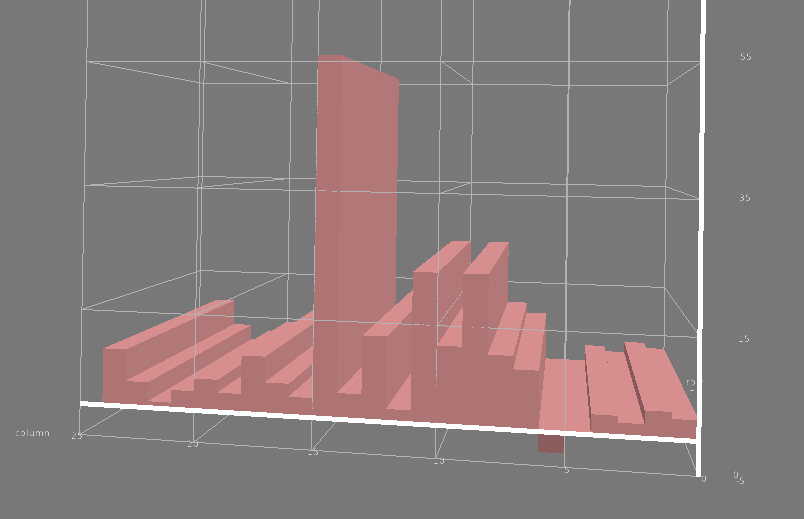
\includegraphics[width=\textwidth]{res/1darray-high-res.png}
    \end{minipage}
\end{figure}

\end{sloppypar}


\end{document}